% ---------------------------------------------------------------
% CV d'Aurélien Chêne - à compiler avec pdfLaTeX (défaut Overleaf)
% Photo facultative~: déposez photo.jpg à côté de main.tex.
% ---------------------------------------------------------------
\documentclass[10pt,a4paper]{article}
\usepackage[utf8]{inputenc}
\usepackage[T1]{fontenc}
\usepackage{helvet}
\renewcommand{\familydefault}{\sfdefault}
\usepackage[a4paper,margin=0pt]{geometry}
\usepackage{xcolor}
\usepackage{tikz}
\usepackage{enumitem}
\usepackage{graphicx}
\usepackage{microtype}

\definecolor{bleu}{HTML}{0B3C8C}
\pagestyle{empty}
\setlength{\parindent}{0pt}

% Titre de section de la barre latérale (blanc, espacé)
\newcommand{\sidetitle}[1]{%
  \vspace{16pt}{\color{white}\bfseries\large\textls[200]{\MakeUppercase{#1}}}\par\vspace{6pt}}
% Titre de section de la colonne principale (bleu, espacé)
\newcommand{\maintitle}[1]{%
  \vspace{9pt}{\color{bleu}\bfseries\large\textls[200]{\MakeUppercase{#1}}}\par\vspace{4pt}}
\SetTracking{encoding={*}, shape=*}{40}

\setlist[itemize]{leftmargin=14pt,itemsep=1pt,topsep=1pt,parsep=0pt,label=\textbullet}
\newlist{sideitems}{itemize}{1}
\setlist[sideitems]{leftmargin=10pt,itemsep=3pt,topsep=2pt,label=\textbullet}

\begin{document}

% Fond bleu de la barre latérale
\begin{tikzpicture}[remember picture,overlay]
  \fill[bleu] (current page.north west) rectangle ([xshift=7.4cm]current page.south west);
\end{tikzpicture}

% ----------------------- BARRE LATÉRALE -----------------------
\begin{minipage}[t][285mm][t]{7.4cm}
  \vspace{0.6cm}
  \hspace{0.9cm}\begin{minipage}{5.7cm}
  \color{white}\small
  \centering
  \IfFileExists{photo.jpg}{%
    \begin{tikzpicture}
      \clip (0,0) circle (1.65cm);
      \node at (0,0) {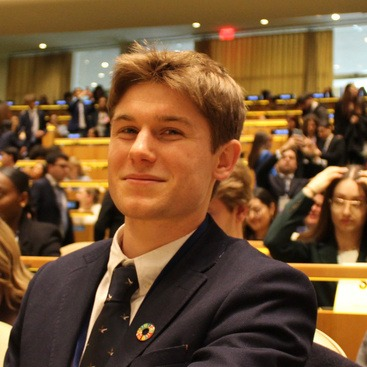
\includegraphics[width=3.3cm]{photo.jpg}};
    \end{tikzpicture}\par}{}
  \raggedright

  \sidetitle{Contact}
  \textbf{Adresse}\\
  2255, rue de l'Université\\
  G1V 0A7, Québec\\
  Canada\par\vspace{6pt}
  \textbf{Courriel}\\
  aurelienchenepro@gmail.com\\
  aurelien.chene.1@ulaval.ca\par\vspace{6pt}
  \textbf{Téléphone}\\
  +33 7 83 07 23 82\\
  +1 (581) 781-5856

  \sidetitle{Compétences}
  \begin{sideitems}\bfseries
    \item Diplomatie
    \item Négociation
    \item Travail d'équipe
    \item Expression orale
    \item Analyse et synthèse
    \item Autonomie
    \item Adaptation
  \end{sideitems}

  \sidetitle{Langues}
  \begin{sideitems}
    \item \textbf{Français}~: langue maternelle
    \item \textbf{Anglais}~: niveau professionnel
    \item \textbf{Espagnol}~: niveau intermédiaire
  \end{sideitems}

  \sidetitle{Intérêts}
  \begin{sideitems}
    \item \textbf{Voile}~: skipper J80, Marine nationale
    \item \textbf{Judo}~: compétition et arbitrage
    \item \textbf{Horlogerie}
  \end{sideitems}
  \end{minipage}
\end{minipage}%
% ----------------------- COLONNE PRINCIPALE -----------------------
\hspace{0.8cm}%
\begin{minipage}[t][285mm][t]{11.3cm}
  \vspace{0.9cm}
  {\color{bleu}\fontsize{26}{28}\selectfont\bfseries AURÉLIEN}\ {\color{bleu}\fontsize{26}{28}\selectfont CHÊNE}\par\vspace{6pt}
  {\small Étudiant en Études internationales, majeure Commerce international et
  investissement, je souhaite intégrer les Missions commerciales de
  l'Université Laval.\par}
  \vspace{3pt}
  {\scriptsize\hfill\begin{minipage}{4.2cm}\raggedleft
  Relations internationales,\\ Géopolitique,\\ Développement économique\end{minipage}\par}

  \maintitle{Formations}
  \small
  \textbf{2025--2026~: Agent au développement international}\\
  Missions commerciales de l'Université Laval, Québec (Canada)
  \begin{itemize}
    \item Réalisation d'une mission commerciale au Japon
    \item Étude de marché
    \item Vente et prospection
    \item Adaptation
  \end{itemize}
  \vspace{5pt}

  \textbf{2025--2027~: Maîtrise en Études internationales -- Commerce international et investissement}\\
  Université Laval, Québec (Canada)
  \begin{itemize}
    \item Commerce
    \item Développement international
    \item Droit
    \item Économie
  \end{itemize}
  \vspace{5pt}

  \textbf{2024--2025~: Délégué ASNUUL -- Membre du Comité «~Social, Humanitarian \& Cultural Issues~» (GA3)}\\
  Association pour la Simulation des Nations Unies de l'Université Laval
  \begin{itemize}
    \item Leadership et diplomatie
    \item Représentation et défense des intérêts d'un État membre
    \item Négociations en anglais
    \item \textbf{Distinction}~: «~Outstanding Delegation Award~» au NMUN 2025
  \end{itemize}
  \vspace{5pt}

  \textbf{2022--2025~: Baccalauréat en science politique}\\
  Université Laval, Québec (Canada)
  \begin{itemize}
    \item \textbf{Études en :} relations internationales, philosophie politique internationale, recherche scientifique
    \item \textbf{Travaux réalisés :} séminaire de recherche «~Franco-Russes~: alliés ou rivaux dans le chaos~»
  \end{itemize}
  \vspace{5pt}

  \textbf{2019--2022~: Baccalauréat général français, section européenne}\\
  Lycée Anne-Marie Javouhey, Brest (France)
  \begin{itemize}
    \item Histoire-géographie, géopolitique et sciences politiques
    \item Sciences économiques et sociales
    \item Mathématiques
  \end{itemize}

  \maintitle{Expérience professionnelle}
  \textbf{2024--2025~: Barman}\\
  Hôtel Maurice, Société Cigar, Québec (Canada)
  \begin{itemize}
    \item Service premium
    \item Trilingue (français, anglais, espagnol)
  \end{itemize}
  \vspace{5pt}

  \textbf{2023--2024~: Gestion de magasin}\\
  Quartz Co, Québec (Canada)
  \begin{itemize}
    \item Relations avec la clientèle
  \end{itemize}
\end{minipage}

\end{document}
